\subsection{Diagramme}
    Hier ein kurzes Beispiel eines Diagramms, dass mit tikz erstellt wurde.\\[1cm]
    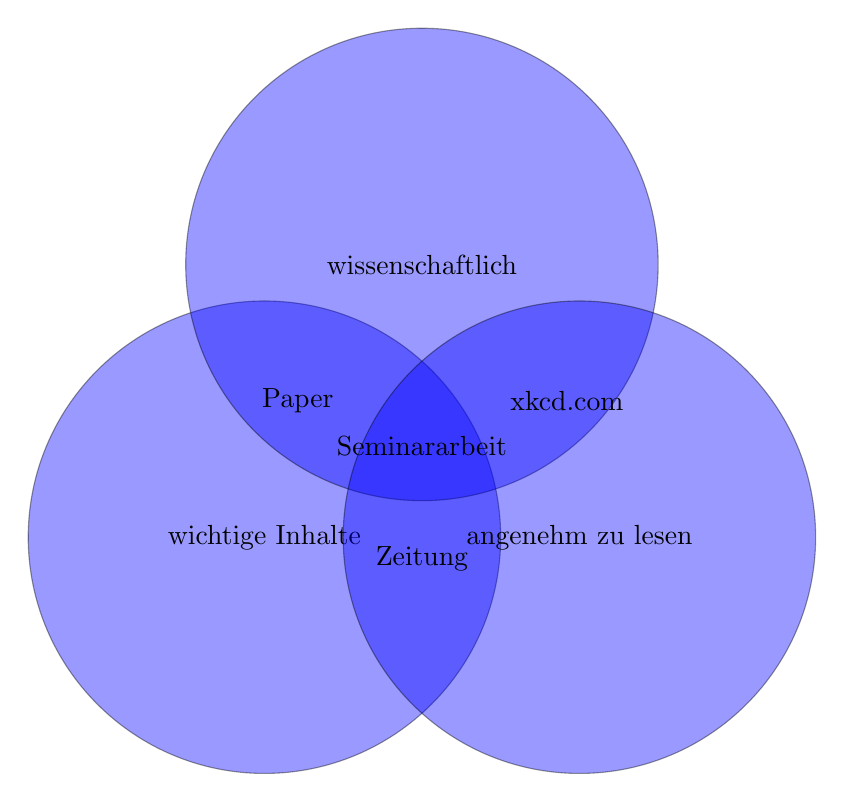
\begin{tikzpicture} [set/.style = {draw,
        circle,
        minimum size = 6cm,
        fill=blue,
        opacity = 0.4,
        text opacity = 1}]
     
    \node (A) [set] {wichtige Inhalte};
    \node (B) at (60:4cm) [set] {wissenschaftlich};
    \node (C) at (0:4cm) [set] {angenehm zu lesen};
     
    \node at (barycentric cs:A=1,B=1) [left] {Paper};
    \node at (barycentric cs:A=1,C=1) [below] {Zeitung};
    \node at (barycentric cs:B=1,C=1) [right] {xkcd.com};
    \node at (barycentric cs:A=1,B=1,C=1) [] {Seminararbeit};
     
    \end{tikzpicture}
    Sie können natürlich auch Diagramme extern erzeugen und als Bild einfügen. Außerdem steht Ihenen bei \href{https://www.mathcha.io/}{mathcha}\footnote[1]{ \href{https://www.mathcha.io/}{https://www.mathcha.io/}} ein Editor für Diagramme und Text zur verfügung.\\
    Wenn Sie Anfangsschwierigkeiten mit \LaTeX{} haben, kann ich Ihnen die Zurhilfenahme dieses Services nur ans Herz legen, da die Dokumente als TeX-Datei exportiert werden können.